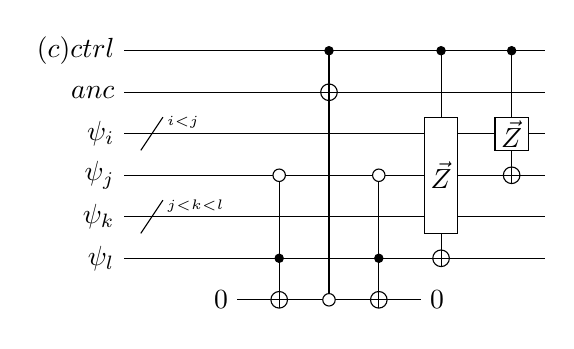
\begin{tikzpicture}[scale=1.000000,x=1pt,y=1pt]
\filldraw[color=white] (0.000000, -7.500000) rectangle (152.000000, 97.500000);
% Drawing wires
% Line 1: ctrl W \text{(c) }ctrl
\draw[color=black] (0.000000,90.000000) -- (152.000000,90.000000);
\draw[color=black] (0.000000,90.000000) node[left] {$\text{(c) }ctrl$};
% Line 2: anc W anc
\draw[color=black] (0.000000,75.000000) -- (152.000000,75.000000);
\draw[color=black] (0.000000,75.000000) node[left] {$anc$};
% Line 3: i W \psi_i
\draw[color=black] (0.000000,60.000000) -- (152.000000,60.000000);
\draw[color=black] (0.000000,60.000000) node[left] {$\psi_i$};
% Line 4: j W \psi_j
\draw[color=black] (0.000000,45.000000) -- (152.000000,45.000000);
\draw[color=black] (0.000000,45.000000) node[left] {$\psi_j$};
% Line 5: k W \psi_k
\draw[color=black] (0.000000,30.000000) -- (152.000000,30.000000);
\draw[color=black] (0.000000,30.000000) node[left] {$\psi_k$};
% Line 6: l W \psi_l
\draw[color=black] (0.000000,15.000000) -- (152.000000,15.000000);
\draw[color=black] (0.000000,15.000000) node[left] {$\psi_l$};
% Line 7: clean0 W 0 0
\draw[color=black] (33.500000,0.000000) -- (114.500000,0.000000);
% Done with wires; drawing gates
% Line 9: i / ^{i<j}
\draw (6.000000, 54.000000) -- (14.000000, 66.000000);
\draw (12.000000, 63.000000) node[right] {$\scriptstyle{^{i<j}}$};
% Line 10: k / ^{j<k<l}
\draw (6.000000, 24.000000) -- (14.000000, 36.000000);
\draw (12.000000, 33.000000) node[right] {$\scriptstyle{^{j<k<l}}$};
% Line 11: ctrl anc i j k l LABEL
% Line 13: clean0 START
\draw[color=black] (41.000000,0.000000) node[fill=white,left,minimum height=15.000000pt,minimum width=15.000000pt,inner sep=0pt] {\phantom{$0$}};
\draw[color=black] (41.000000,0.000000) node[left] {$0$};
% Line 14: -j l +clean0
\draw (56.000000,45.000000) -- (56.000000,0.000000);
\draw[fill=white] (56.000000, 45.000000) circle(2.250000pt);
\filldraw (56.000000, 15.000000) circle(1.500000pt);
\begin{scope}
\draw[fill=white] (56.000000, 0.000000) circle(3.000000pt);
\clip (56.000000, 0.000000) circle(3.000000pt);
\draw (53.000000, 0.000000) -- (59.000000, 0.000000);
\draw (56.000000, -3.000000) -- (56.000000, 3.000000);
\end{scope}
% Line 15: ctrl +anc -clean0
\draw (74.000000,90.000000) -- (74.000000,0.000000);
\filldraw (74.000000, 90.000000) circle(1.500000pt);
\begin{scope}
\draw[fill=white] (74.000000, 75.000000) circle(3.000000pt);
\clip (74.000000, 75.000000) circle(3.000000pt);
\draw (71.000000, 75.000000) -- (77.000000, 75.000000);
\draw (74.000000, 72.000000) -- (74.000000, 78.000000);
\end{scope}
\draw[fill=white] (74.000000, 0.000000) circle(2.250000pt);
% Line 16: -j l +clean0
\draw (92.000000,45.000000) -- (92.000000,0.000000);
\draw[fill=white] (92.000000, 45.000000) circle(2.250000pt);
\filldraw (92.000000, 15.000000) circle(1.500000pt);
\begin{scope}
\draw[fill=white] (92.000000, 0.000000) circle(3.000000pt);
\clip (92.000000, 0.000000) circle(3.000000pt);
\draw (89.000000, 0.000000) -- (95.000000, 0.000000);
\draw (92.000000, -3.000000) -- (92.000000, 3.000000);
\end{scope}
% Line 17: clean0 END
\draw[color=black] (107.000000,0.000000) node[fill=white,right,minimum height=15.000000pt,minimum width=15.000000pt,inner sep=0pt] {\phantom{$0$}};
\draw[color=black] (107.000000,0.000000) node[right] {$0$};
% Line 19: i j k G $\vec{Z}$ +l ctrl
\draw (114.500000,90.000000) -- (114.500000,15.000000);
\begin{scope}
\draw[fill=white] (114.500000, 45.000000) +(-45.000000:8.485281pt and 29.698485pt) -- +(45.000000:8.485281pt and 29.698485pt) -- +(135.000000:8.485281pt and 29.698485pt) -- +(225.000000:8.485281pt and 29.698485pt) -- cycle;
\clip (114.500000, 45.000000) +(-45.000000:8.485281pt and 29.698485pt) -- +(45.000000:8.485281pt and 29.698485pt) -- +(135.000000:8.485281pt and 29.698485pt) -- +(225.000000:8.485281pt and 29.698485pt) -- cycle;
\draw (114.500000, 45.000000) node {$\vec{Z}$};
\end{scope}
\begin{scope}
\draw[fill=white] (114.500000, 15.000000) circle(3.000000pt);
\clip (114.500000, 15.000000) circle(3.000000pt);
\draw (111.500000, 15.000000) -- (117.500000, 15.000000);
\draw (114.500000, 12.000000) -- (114.500000, 18.000000);
\end{scope}
\filldraw (114.500000, 90.000000) circle(1.500000pt);
% Line 20: i G $\vec{Z}$ +j ctrl
\draw (140.000000,90.000000) -- (140.000000,45.000000);
\begin{scope}
\draw[fill=white] (140.000000, 60.000000) +(-45.000000:8.485281pt and 8.485281pt) -- +(45.000000:8.485281pt and 8.485281pt) -- +(135.000000:8.485281pt and 8.485281pt) -- +(225.000000:8.485281pt and 8.485281pt) -- cycle;
\clip (140.000000, 60.000000) +(-45.000000:8.485281pt and 8.485281pt) -- +(45.000000:8.485281pt and 8.485281pt) -- +(135.000000:8.485281pt and 8.485281pt) -- +(225.000000:8.485281pt and 8.485281pt) -- cycle;
\draw (140.000000, 60.000000) node {$\vec{Z}$};
\end{scope}
\begin{scope}
\draw[fill=white] (140.000000, 45.000000) circle(3.000000pt);
\clip (140.000000, 45.000000) circle(3.000000pt);
\draw (137.000000, 45.000000) -- (143.000000, 45.000000);
\draw (140.000000, 42.000000) -- (140.000000, 48.000000);
\end{scope}
\filldraw (140.000000, 90.000000) circle(1.500000pt);
% Done with gates; drawing ending labels
% Done with ending labels; drawing cut lines and comments
% Done with comments
\end{tikzpicture}
